% -*-cap2.tex-*-
% Este fichero es parte de la plantilla LaTeX para
% la realización de Proyectos Final de Carrera, protegido
% bajo los términos de la licencia GFDL.
% Para más información, la licencia completa viene incluida en el
% fichero fdl-1.3.tex

% Copyright (C) 2009 Pablo Recio Quijano 

\section{Resultados obtenidos}

Los resultados obtenidos gracias al desarrollo de esta aplicación han sido tremendamente satisfactorios, tanto en el
plano personal como en el profesional. \\

Como hitos conseguidos podemos destacar los siguientes:

\subsection{Primer simulador de dominó libre}

Sin querer resultar pretencioso --- y siempre según la investigación previa que hemos realizado --- Dominous es el primer
videojuego de dominó internacional bajo licencia libre, con todas las ventajas que ello conlleva:

\begin{itemize}
    \item Posibilidad de que pueda ser mejorado por la comunidad~\cite{raymond01a}, añadiendo soluciones a errores de código o refactorizaciones, proporcionando nuevos jugadores, mejorando el sistema y motor de Inteligencia Artificial, añadiendo nuevas
        funcionalidades que se encuentran fuera de los requisitos iniciales del proyecto, portar Dominous a otros
        entornos, Sistemas Operativos o incluso consolas de videojuegos...
    \item Libertad para aprender mediante la lectura de la documentación del proyecto o del análisis del código~\cite{sobre_swlibre_2004}.
    \item Facilidad para llegar a más usuarios gracias a la gratuidad del producto y su disponibilidad en Internet.
\end{itemize}

El acto de volcar todo el conocimiento de esta aplicación a la comunidad --- código, documentación o arte, por ejemplo --- es desde
mi punto de vista un acto lógico y natural de intentar devolver a la comunidad del software libre una pequeña 
parte de todo lo que se ha obtenido de ella. Con un pequeño repaso a las herramientas utilizadas podemos comprobar
que la gran mayoría de ellas tienen licencias libres, y gracias a ellas hemos podido desarrollar esta aplicación con éxito,
pudiendo elegir entre un gran número de diferentes opciones y tomando la que mejor nos conviene en cada momento.


\subsection{Aplicación de lo aprendido en la carrera}

Existe una creencia extendida sobre que los estudios universitarios técnicos suelen pecar de facilitar conocimientos que
resultan muy teóricos, con muy poca aplicación práctica a la hora de desarrollar un proyecto real, así que es muy
gratificante poder comprobar que gracias todas las asignaturas de la carrera se consigue un fuerte bagaje y una metodología
de trabajo que nos permite llevar a cabo proyectos de gran envergadura como este. \\

La principal asignatura que nos ha permitido solventar los principales problemas de este proyecto ha sido la de Inteligencia
Artificial, impartida por el profesor Don Ignacio Pérez Blanquer, en especial el apartado de análisis de juegos. Los apartados
sobre representación del conocimiento y la base teórica sobre sistemas expertos también han resultado de gran ayuda. \\

Por otro lado, gracias a las asignaturas relacionadas con la Ingeniería del Software se han podido definir las líneas
maestras que gobiernan el desarrollo de la aplicación, afrontando el proyecto con mucha más seguridad y confianza en la
buena terminación del mismo. \\

Y por supuesto, no podemos olvidar las asignaturas de Análisis y Diseño de Algoritmos, Estructura de Datos, Programación
orientada a Objetos, Sistemas Operativos y tantas otras que, además de enseñar conocimientos, enseñan cómo pensar y
cómo aprender, lo cual es mucho más importante que el simple hecho del conocimiento en sí o aprobar simplemente la asignatura.


\subsection{Aprendizaje del juego de dominó}

Debo reconocer que, cuando mi tutor de proyecto me presentó esta idea, creía que el dominó era un juego sencillo y
fácilmente abarcable con las herramientas de Inteligencia Artificial que conocemos hoy día. Y nada más lejos de la realidad. \\

Al principio pensaba que el dominó se limitaba a gestionar tus fichas dentro de un radio de acción muy limitado --- ya
que, comparado con otros juegos como el ajedrez, en éste no podemos colocar o mover la ficha que queramos, sino 
solamente mover una del pequeño subconjunto formado por las fichas candidatas a colocarse --- pero mediante la lectura
de libros de estrategias y partidas comentadas empecé a ver las dificultades que entraña el jugar una buena partida
de dominó. El dominó es un juego muy profundo, con una componente de suerte mucho más pequeña de lo que la gente cree,
mucha psicología, estrategias, tácticas, y sobre todo mucha, mucha diversión. \\

%Porque el dominó es más que un simple juego, y eso supera la dimensión de Inteligencia Artificial que pueda tener el proyecto. \\

El dominó es un juego social y de caballeros, que bien jugado afianza y genera confianza y compañerismo entre los jugadores
y parejas. Es un juego con reglas simples pero estrategias complejas, que fortalece la memoria (recordando o intentando
recordar los diferentes movimientos que ha realizado cada jugador) y cuya diversión se dispara al contar con un compañero,
ya que el juego en equipo --- sin posibilidad de comunicación entre ellos --- añade mucha complejidad y humanidad a un
juego que dista muchísimo de estar basado simplemente en estadística o probabilidades. \\

Y gracias a todo lo aprendido ahora puedo observar el mundo del dominó con otra mirada y, por supuesto, respetar y admirar
a los grandes jugadores de dominó.

\subsection{Primer proyecto que realizo de manera íntegra}


Para un estudiante de Ingeniería Informática es una gran satisfacción realizar un proyecto de manera completa, para lo cual
se han tenido que aplicar conocimientos de muchas ramas, y ha sido muy divertido mezclar la programación pura y dura
de la aplicación con conocimientos más amplios como pueden ser:

\begin{description}
    \item[Diseño gráfico] A la hora de hacer un videojuego un apartado tremendamente importante es el aspecto visual del mismo.
        En multitud de ocasiones los ingenieros informáticos caemos en la trampa de hacer aplicaciones que solventan
        los problemas concretos, pero que fallan a la hora de ser atractivos para el usuario final. Y si no hay usuario
        final o no le resulta atractivo y no lo usa, la aplicación no tendrá sentido. 

        Para diseñar el aspecto visual se han definido unas líneas maestras generales y se ha intentado ser consistente
        con este estilo visual, para dotar de uniformidad y coherencia a la aplicación; los botones tienen el mismo diseño
        durante toda la aplicación, la tipografía utilizada se limita únicamente a dos fuentes, la paleta de color
        también se mantiene constante, etcétera. 

        Por otro lado, ya que no somos estudiantes de bellas artes ni se puede presuponer que un ingeniero informático
        debe tener conocimientos de diseño gráfico, he optado por una solución que ha dado muy buenos resultados, y es
        el utilizar una interfaz y diseño minimalista, con líneas y fondos claros, ciñéndonos a jugar con tonos de color
        blanco, gris, negro y amarillo --- para dotar de una fuerte uniformidad de estilo --- y sin buscar en ningún
        momento la espectacularidad gráfica o visual. Gracias a esta solución hemos conseguido que la aplicación no
        resulte confusa ni pesada, sea legible y tenga un aspecto gráfico bastante profesional.

\item [Música y efectos de sonido] La música también juega un papel importante en un videojuego, esta aplicación está orientada a un
        público muy general, y el ritmo del juego es tranquilo y pausado, así que se eligió el jazz libre como estilo base
        para acompañar al juego. En cuanto a los efectos de sonido, se grabaron golpes reales de fichas de dominó sobre una mesa y aletoriamente se producen al poner fichas en el juego.
        
    \item[Gestión de proyectos] Para gestionar satisfactoriamente el proyecto se contó con herramientas profesionales
        como sistemas de control de versiones (SVN), aplicaciones de ticketing para asignar y crear tareas, una página
        web en la que volcar la información y documentación que se iba generando, aplicaciones de screencast para
        animar a la comunidad a participar o Latex y Dia para diseño de documentación y diagramas, entre otros muchos.

    \item[Usabilidad y Experiencia de Usuario] Se ha intentado aplicar mucho sentido común e iteraciones al diseño de la
        interfaz de la aplicación, para que su facilidad de uso sea un aliciente para usarlo, y no un escollo que
        dificulte el acceso a ella.

\end{description}

\section{Trabajos futuros}

A la hora de establecer los requisitos técnicos de un proyecto fin de carrera se puede caer en la tentación de querer desarrollar y
especificar un proyecto que no sea realista con las limitaciones técnicas, de tiempo y de recursos que se disponen para la
realización del mismo. \\

Este acto puede resultar más flagrante en el caso de que el alumno se sienta muy atraído con el mismo --- como es el caso
que nos ocupa en este momento --- ya que el placer y el interés de desarrollar un producto profesional, similar a los que
se pueden encontrar en el mercado, puede llevarnos a una gran frustración por no conseguirlo. Debemos tener en cuenta de que
los estudios profesionales de videojuegos hoy en día cuentan con una gran cantidad de recursos, tanto de tiempo como
económicos, además de aglutinar profesionales de diferentes áreas (como puede ser el diseño gráfico, directores de arte,
expertos en usabilidad o programadores de bajo nivel, por nombrar algunos) y querer conseguir un producto de condiciones
similares es disparatado. \\

Es por estas razones que varias funcionalidades han debido de quedarse --- lamentablemente --- fuera del pliego de
especificaciones de requisitos. Aún así nos gustaría comentarlas a continuación, para que, por un lado, quede constancia
del trabajo de estudio preliminar del sector que se ha realizado y, por otro lado, por si alguien quiere recoger
el guante y continuar añadiendo nuevas funcionalidades al proyecto, mostrar un conjunto de pasos o características
muy interesantes de implementar:

\subsection{Juego en red}

En la fase de especificación de requisitos se barajó la opción de que Dominous presentara opciones para desarrollar una
partida en red, pero después de un profundo análisis se desechó esta opción; el juego en red plantea varias problemáticas
que resultan verdaderamente dificultosas y que explicamos a continuación:

\begin{itemize}
    \item La principal razón es que existe el problema conceptual de desarrollar una partida a un juego con conocimiento parcial 
        de forma remota --- la base del dominó reside en que los jugadores no pueden conocer las fichas de sus compañeros,
        y si la partida se juega en red nada impide que los equipos intercambien información mediante otras vías de
        comunicación.

        Se podría argumentar que depende del jugador y de la moral y ética que lo gobierne el utilizar estas trampas
        para conseguir una victoria de forma poco correcta, y que el videojuego no debe entrar en este terreno, pero
        es cierto que dejar una puerta abierta a este tipo de jugadores es crear un juego con un gran fallo conceptual,
        que no permitiría las principales premisas de la aplicación, que son entretener y enseñar el mundo del dominó.

    \item Tampoco hay que olvidar que, al ofrecer este tipo de juego, estamos cambiando los objetivos principales del
        juego, que es conseguir profundizar en el mundo de la Inteligencia Artificial orientado al dominó.

    \item Finalmente tampoco podemos obviar las limitaciones técnicas y de escasez de mercado, que nos obligaría en
        principio a tener que desarrollar la aplicación para otro tipo de medios con más proyección --- como podría
        ser dispositivos móviles, aplicaciones en flash o directamente orientado a web --- y que obligaría a reorientar
        todo el desarrollo del proyecto.
\end{itemize}

\subsection{Servidor web para compartir sistemas expertos}

También sería muy interesante poder ofrecer una forma de disponer de los diferentes sistemas expertos de forma remota.
Así sería sencillo poder realizar torneos entre diferentes jugadores y equipos, cada uno programado por un participante
del torneo. \\

Para ello sería necesario buscar un formato estándar de compartición de sistemas expertos basados en Dominous, desarrollando
unas especificaciones lo suficientemente generales para dar potencia al la Inteligencia Artificial, y relativamente
simple para que no suponga una curva de aprendizaje agresiva al nuevo jugador. \\

Todo esto sin olvidar que es necesario que la ejecución de los sistemas expertos se realice en la misma máquina; ya que
si se facilita una API para comunicación con otros sistemas estaríamos cayendo en el mismo error que en el juego en red, 
esto es, permitiendo que equipos pudieran utilizar canales de comunicación alternativos y jugar con ventaja frente a otros.

\subsection{Analizador de partidas con aprendizaje automático o semiautomático}

Existen multitud de herramientas de Inteligencia Artificial orientadas a simular sistemas expertos, comportamientos y 
y razonamiento humano. Una de ellas es el \textbf{aprendizaje automático}; sería un proyecto muy interesante generar un sistema
que reciba como entrada ficheros con históricos de partidas --- como las que genera Dominous, por ejemplo --- y obtenga
información mediante el análisis de cada movimiento, dependiendo de la posición del jugador en la mesa y de las fichas
existentes en cada mano. \\

Para conseguir este fin se podrían utilizar técnicas como las redes neuronales o árboles de decisión. Y si se quiere
dar un paso más se podría apoyar en aprendizaje supervisado --- utilizando a algún experto real en el mundo del dominó
que evalúe los posibles movimientos, animando o corrigiendo según la valoración del mismo y creando un sistema que
vaya mejorando con cada uso.

\subsection{Migración de la aplicación a otros sistemas}

Dominous se ha programado con los requisitos de correcto funcionamiento bajo sistemas operativos basados en GNU/Linux (como
Ubuntu) y Microsoft Windows, pero sería un proyecto interesante intentar migrar el sistema a otros entornos como podrían ser
dispositivos móviles, consolas portátiles o tablets. \\

\begin{figure}[h]
  \begin{center}
    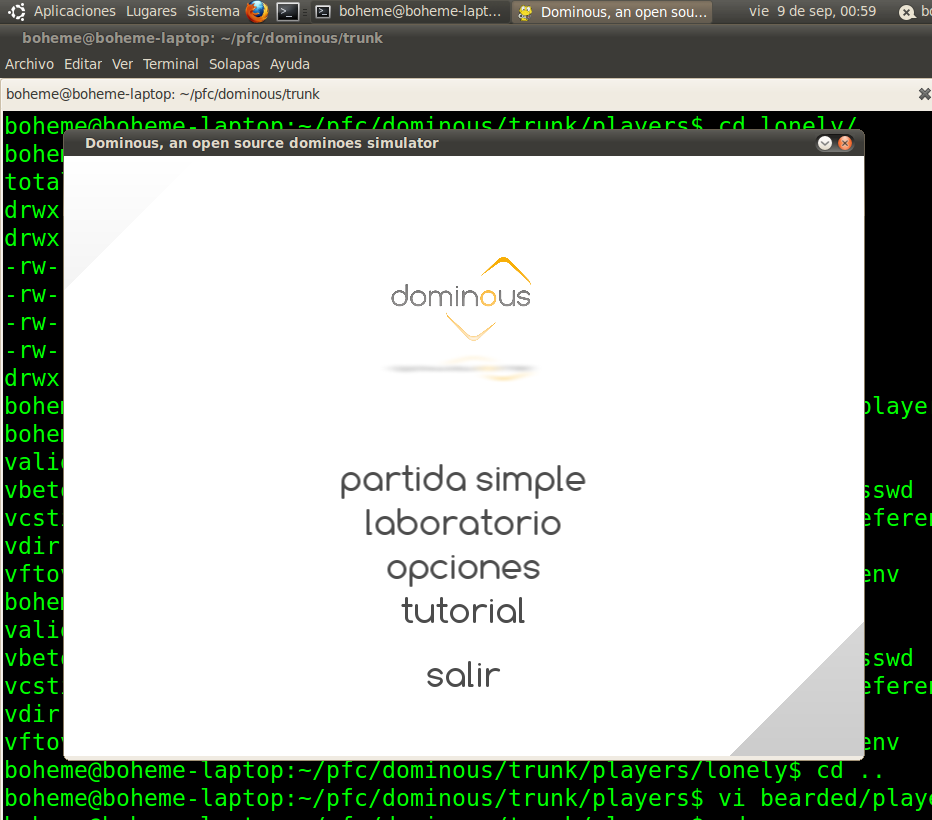
\includegraphics[scale=0.7]{dominous_ubuntu.png}
  \end{center}
  \caption{Dominous ejecutándose en un entorno GNU/Linux, distribución Ubuntu 10.04}
  \label{dominous_ubuntu}
\end{figure}


\begin{figure}[h]
  \begin{center}
    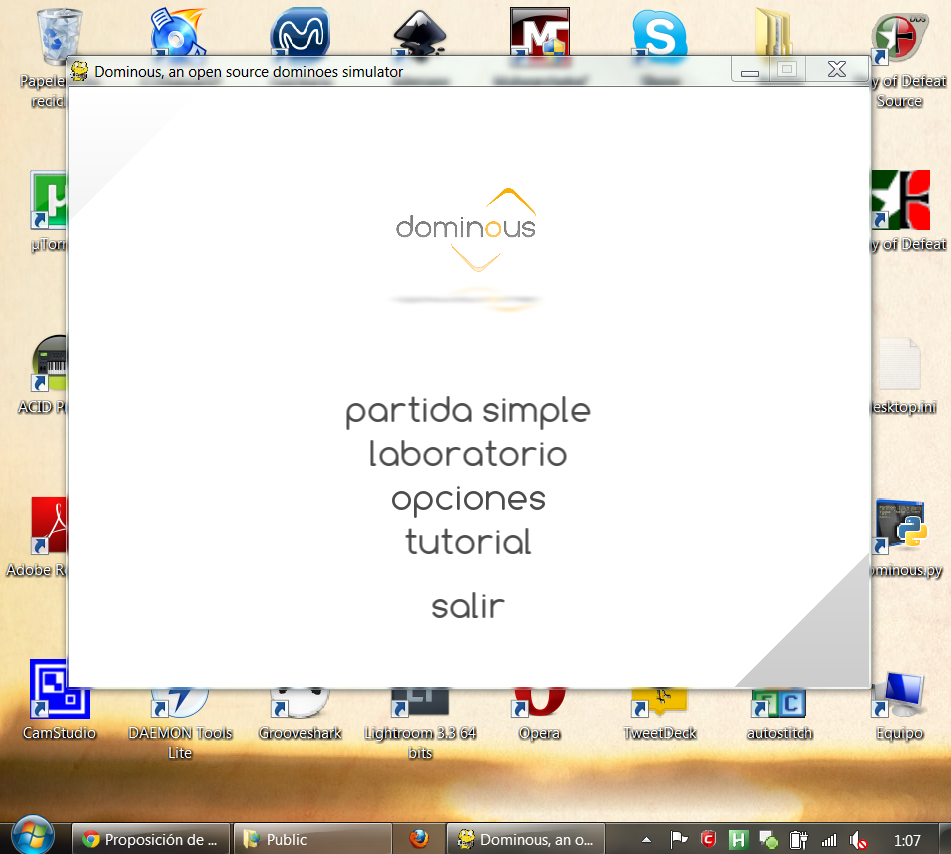
\includegraphics[scale=0.7]{dominous_windows.png}
  \end{center}
  \caption{Dominous ejecutándose en un entorno Microsoft Windows 7}
  \label{dominous_windows}
\end{figure}

